\begin{thwbr}
\chapter{Debian GNU/Linux}\label{chap:debian}
หนังสือเล่มนี้เลือกใช้ Debian GNU/Linux เป็นลินุกซ์ดิสทริบิวชันอ้างอิงเนื่องจากเหตุผลหลายๆอย่างและในบทนี้จะแนะนำการติดตั้ง Debian และการจัดการแพ็กเกจซอฟต์แวร์เพื่อที่จะให้ผู้ใช้คุ้นเคยและนำไปใช้งานได้จริงต่อไป.

\section{ติดตั้ง Debian GNU/Linux}

ขั้นตอนการติดตั้งลินุกซ์ไม่ว่าจะเป็นดิสทริบิวชันใดก็ตามโดยทั่วไปมีขั้นตอนดังนี้.
\begin{enumerate}
\item ดาวน์โหลดซีดีในรูปของไฟล์อิมเมจ ISO
\item เขียนซีดีรอม และบูตเครื่องคอมพิวเตอร์จากซีดีรอม
\item ติดตั้งระบบปฏิบัติการลินุกซ์ด้วยโปรแกรมติดตั้งของดิสทริบิวชันที่ใช้
\item ปรับแต่งและอัปเดทซอฟต์แวร์
\end{enumerate}

\section{ดาวน์โหลดซีดี}
การติดตั้งลินุกซ์โดยทั่วไปมักจะใช้ซีดีรอมเป็นสื่อในการติดตั้ง. ผู้ใช้สามารถซื้อหรือจะดาวน์โหลดด้วยตัวเองจากเว็บไซด์ของดิสทริบิวชันต่างๆ.

ซีดีที่ดาว์นโหลดมาจะอยู่ในรูปของไฟล์ที่เรียกว่า\emph{ดิสก์อิมเมจ (disk image)} และมักจะมีส่วนขยายชื่อไฟล์เป็น \cmd{.iso}. %
\mymemo{ส่วนขยายชื่อไฟล์ \cmd{.iso} เป็นแค่ชื่อที่ให้คนอ่านแล้วเข้าใจ. จริงๆแล้วไม่จำเป็นต้องเป็น \cmd{.iso}, บ้างก็ใช้ส่วนขยายชื่อไฟล์เป็น \cmd{.raw}, {\latintext\tt .img} หรือไม่ใส่ส่วนขยายชื่อไฟล์.}%

ในเว็บไซด์หน้าดาว์นโหลดซีดี Debian \footnote{http://www.debian.org/CD} จะมีบอกวิธีการดาว์นโหลดหลายแบบเช่นดาวน์โหลดด้วย jigdo\gindex{jigdo} ซึ่งเป็นโปรแกรมพิเศษสำหรับดาว์นโหลดไฟล์ ISO ของ Debian, ดาวน์โหลดโดยใช้ Bittorrent. แต่วิธีที่เข้าใจง่ายที่สุดคือดาว์นโหลดผ่านทาง FTP หรือ HTTP โดยไปที่หน้าดาว์นโหลด Debian CD/DVD ผ่านทาง HTTP/FTP\footnote{http://www.debian.org/CD/http-ftp/} ก่อน. จากนนั้นก็เลือก FTP หรือ HTTP ที่ใกล้ตัวเพื่อความรวดเร็วในการดาว์นโหลด. 

ตัวอย่างเช่นถ้าดาว์นโหลดจาก \mbox{ftp://cdimage.debina.org/debian-cd/3.1\_r0a/i386/iso-cd/} จะมีไฟล์ \cmd{.iso} หลายตัวให้เลือก. ให้เลือกดาว์นโหลดไฟล์ debian-31r0a-i386-binary-1.iso ไฟล์เดียวก็พอเพียงสำหรับการติดตั้ง. ไฟล์อิมเมจนี้สามารถใช้ติดตั้งโดยไม่มีเน็ตเวิร์กได้และมีแพ็กเกจพื้นฐานที่จำเป็นรวมถึงสภาพแวดล้อมเดสก์ท็อปให้ด้วย. ไฟล์ debian-31r0a-i386-businesscard.iso เป็นไฟล์อิมเมจสำหรับ CD ขนาดนามบัตรซึ่งแพ็กเกจที่อยู่อิมเมจก็จะน้อยลง. และไฟล์ debian-31r0a-i386-netinst.iso เป็นไฟล์อิมเมจสำหรับติดตั้งโดยผ่านเน็ตเวิร์กซึ่งแพ็กเกจที่ติดตั้งจะดาว์นโหลดผ่านเน็ตเวิร์กขณะติดตั้ง.



\subsection{การตรวจสอบดิสก์อิมเมจ}
ไฟล์ดิสก์อิมเมจที่ดาวน์โหลดมามักจะมีขนาดใหญ่ประมาณ 700 MB เพื่อเขียนลงซีดีรอมหนึ่งแผ่น. การดาวน์โหลดไฟล์ใหญ่แบบนี้อาจจะเกิดความผิดพลาดในการโอนถ่ายข้อมูล, ซึ่งบางครั้งนำไฟล์ที่ดาวน์โหลดไปเขียนซีดีแล้วใช้งานไม่ได้. ในบางกรณีที่ผู้ใช้ไม่ได้ดาวน์โหลดไฟล์จากเว็บไซด์ของดิสทริบิวชันอย่างเป็นทางการ, อาจจะมีผู้ไม่ประสงค์ดีแอบใส่โปรแกรมที่ไม่พึงประสงค์ลงไปในไฟล์ติดตั้งด้วย. ด้วยเหตุผลเหล่านี้เองผู้ใช้จึงควรตรวจสอบไฟล์ดิสก์อิมเมจที่ดาวน์โหลดมาก่อนใช้งาน.

ผู้ใช้สามารถตรวจสอบไฟล์ที่ดาวน์โหลดมาด้วยโปรแกรม \cmd{md5sum}. %
%
\begin{MyVerbatim}
$ \cin{md5sum debian-31r0a-i386-binary-1.iso}
b49a7955be5e286eff873a9bd157793a  debian-31r0a-i386-binary-1.iso
\end{MyVerbatim}
%$
โปรแกรม \cmd{md5sum} จะแสดงค่า\emph{เช็คซัม (checksum)} ของไฟล์ที่ต้องการตรวจสอบ. เมื่อได้ค่าเช็คซัมแล้วก็นำไปเทียบกับค่าเช็คซัมที่ดิสทริบิวชันแสดงไว้ว่าตรงกันหรือไม่. ปรกติไซด์ที่ดาว์นโหลดจะมีไฟล์ \cmd{MD5SUMS} ให้ดาว์นโหลดด้วย. ไฟล์นี้จะมีค่าเช็คซัมของไฟล์อิมเมจไว้ให้ดูเปรียบเทียบว่าค่าตรงกันหรือไม่. ถ้าไม่ตรงกันแสดงว่าไฟล์ที่ดาวน์โหลดมามีข้อมูลไม่ตรงกับต้นฉบับจริง. %ดิสทริบิวชันมักจะเตรียมไฟล์รายการค่าเช็คซัมกับชื่อไฟล์ไว้ให้ดาวน์โหลดด้วยเพื่อที่ผู้ใช้จะได้ตรวจสอบได้ว่าไฟล์ที่ดาวน์โหลดไปถูกต้องหรือไม่.


สำหรับผู้ที่ใช้วินโดวส์และต้องการตรวจค่าเช็คซัม, ให้ใช้โปรแกรม MD5summer \cite{md5summer} ซึ่งเป็นซอฟต์แวร์เสรี.

\section{การเขียนซีดี}
โปรแกรมที่ใช้เขียนซีดีบนลินุกซ์มีหลายโปรแกรมให้เลือกใช้เช่น \cmd{xcdroast}, \cmd{gtoaster} แต่โปรแกรมเหล่านี้ต่างก็เป็น frontend ของโปรแกรม (คำสั่ง) \cmd{cdrecord} ทั้งนั้น. เมื่อดาวน์โหลดัและตรวจสอบไฟล์ที่ดาวน์โหลดแล้ว, ให้ใช้คำสั่ง \cmd{cdrecord}. 

\myexplanation{cdrecord}{\cmd{dev=0,0,0} เป็นการระบุดีไวส์ซีดี. \cmd{-eject} ให้คอมพิวเตอร์ดีดตัวซีดีออกจากไดรว์เมื่อเขียนซีดีเสร็จ. และ \cmd{speed=4} เป็นการใช้ความเร็ว 4 เท่า.}
\begin{MyVerbatim}
# \cin{cdrecord dev=0,0,0 -eject speed=4 samila-5.5-i386-cd1.iso}
\end{MyVerbatim} 

ผู้ที่ใช้วินโดวส์สามารถใช้โปรแกรมเขียนไฟล์ \cmd{.iso} ลงซีดีได้เช่น Nero, Easy CD Creator ฯลฯ.  หรือถ้าเป็นซอฟต์แวร์เสรีสามารถใช้ BurnAtOnce\footnote{http://www.burnatonce.com}, CDBruenerXP Pro\footnote{http://www.cdburnerxp.se} ฯลฯ.
\section{การติดตั้งลินุกซ์}
ก่อนอื่นให้ตรวจสอบ BIOS ของคอมพิวเตอร์ให้เครื่องคอมพิวเตอร์บูตเครื่องจากซีดีได้. จากนั้นให้ใส่ซีดีแล้วเปิดเครื่องใหม่, ถ้าไม่มีข้อผิดพลาดใดๆก็จะสามารถบูตจากแผ่นซีดีได้.

\subsubsection*{ตั้งค่า BIOS}\mymemo{เข้าหน้าจอ BIOS และเปลี่ยนให้เครื่องบูตจาก CDROM. วิธีตั้งให้เครื่องเข้า BIOS อาจจะกด \cmd{F1}, \cmd{Del}, \cmd{ESC} แล้วแต่กรณี. หลังจากที่เข้า BIOS แล้งแก้เมนูการบูตให้บูตจาก CDROM, บันทึกการแก้ไขแล้วรีบูต.}
\bigskip
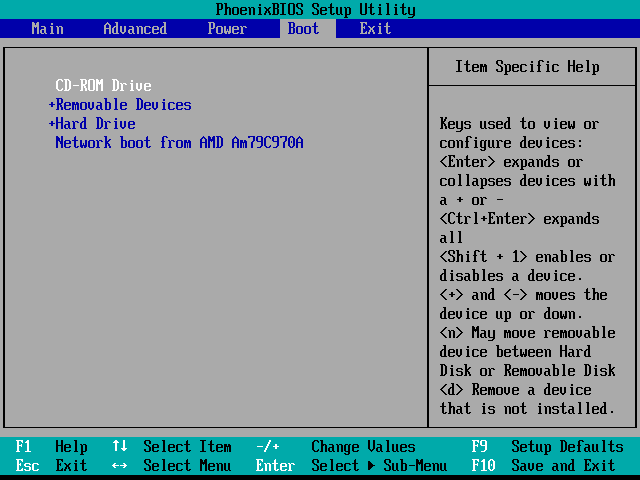
\includegraphics[scale=.45]{bios-cdrom.eps}

\vfill



\subsubsection*{เข้าสู่โปรแกรมติดตั้ง}%\mymemo{ผู้อ่านสามารถเลือกวิธีการติดตั้ง (อินเทอร์เฟส) ได้สองแบบคือแบบกราฟฟิกและแบบเท็กซ์โหมด. ในที่นี้จะอธิบายวิธีการติดตั้งแบบกราฟฟิก. หากต้องการติดตั้งในระบบเท็กซ์โหมด, ให้พิมพ์ \cmd{linux text} แล้วกดคีย์ Enter. การติดตั้งแบบกราฟฟิกให้กดคีย์ Enter เพื่อดำเนินการต่อไป. 
%
%นอกจากการติดตั้งแล้วผู้อ่านสามารถใช้แผ่นซีดีเป็นแผ่นบูตคอมพิวเตอร์แก้ไขปัญหาเวลาเครื่องบูตไม่ได้. ในกรณีนี้เรียกว่าการบูตแบบ Rescue. นอกจากนั้นผู้อ่านสามารถเลือกวิธีการติดตั้งจากเน็ตเวิร์คได้ด้วย.}
\mymemo{หนังจากที่ใส่แผ่น CD แล้วบูตจากจะมีหน้าจอดังภาพ. ให้กดคีย์ \cmd{Enter} หรือกดคีย์ \cmd{F1} เพื่อดูคำอธิบายช่วยเหลือ.}

\bigskip
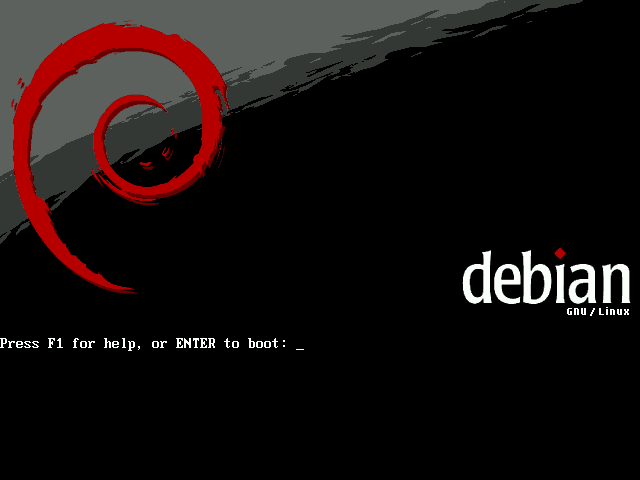
\includegraphics[scale=.45]{debian-cd-boot.eps}

\vfill
%\subsubsection*{หน้าจอต้อนรับของโปรแกรมติดตั้ง}\mymemo{ด้านซ้ายมือของหน้าจอจะเป็นหน้าต่างช่วยเหลือ, ช่วยอธิบายขั้นตอนการติดตั้ง. ในช่วงนี้ผู้อ่านสามารถกดปุ่มอ่าน\emph{รีลีสโน้ต (release note)} ซึ่งจะแนะนำความสามารถใหม่ในลินุกซ์ทะเล. ให้กดปุ่ม ``ถัดไป'' เพื่อดำเนินการต่อไป.}%

... to be continued


\end{thwbr}
\wbrin

